\chapter{Results and Discussions}

The results of the experiments performed on the NPSC modules are given and described in this section. Results belonging to the same category are firstly described and a discussion on the outcome of the experiment is done on each result and on the category to see whether or not the results converge. 

%%%%%%%%%%%%%%%%%%%%%%%%%%%%%%%%%%%%%%%%%%%%%%%%%%%%%%%%%%%%%%%%%%%%%%%%%%%%%%%%%%%%
% SECTION: Hardware module tests
%%%%%%%%%%%%%%%%%%%%%%%%%%%%%%%%%%%%%%%%%%%%%%%%%%%%%%%%%%%%%%%%%%%%%%%%%%%%%%%%%%%%
\section{Hardware module tests}
This section provides the result of the hardware serial communication protocol. Each result is compared to the theoretical communication protocol of its corresponding hardware module. 

\subsection{DS1307}
The external RTC (DS1307) was tested by writing the value of 5 to its minute memory register. The serial information generated by the I2C pins are displayed in \cref{coms_ds1307}. The clock serial information is observed at channel 0 and the data serial information is observed at channel 1. The logic analyser was set to analyse the data using the I2C protocol, the interpretation of the data is displayed above the SDA serial data.
\begin{figure}[h!]
	\centering
	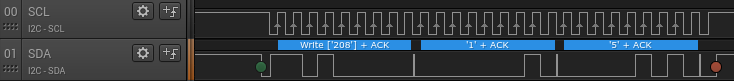
\includegraphics[scale=0.6]{coms_ds1307.png}
	\caption{Serial information sent to the external RTC when setting the minute to 5.}
	\label{coms_ds1307}
\end{figure}
\subsubsection{Discussion}
The I2C protocol is started when the SDA changes state going from high to low while the SCL line is high, this is indicated by the green dot on SDA line. The address of the DS1307 is then sent with an extra 0 bit indicating that a write action is required ($Write['208']$)). The address of the minute registered is then sent ($'1'$) and finally, the data is written to the register ($'5'$). Note that each instruction sent is acknowledged ($+ACK$) by the DS1307.

\subsection{25LC640}
The EEPROM (25LC640) was tested by writing a value of 10 at its first address. The serial information generated by the 25LC640 pins are displayed in \cref{fig:coms_25lc640}. The MOSI, MISO, CLK, and EN serial information are respectively observed at channel 0,1,2, and 3. The logic analyser was set to analyse the data using the SPI protocol, the interpretation of the data is displayed above the MOSI and MISO serial data.
\begin{figure}[h!]
	\centering
	\begin{minipage}[b]{\textwidth}
		\centering
		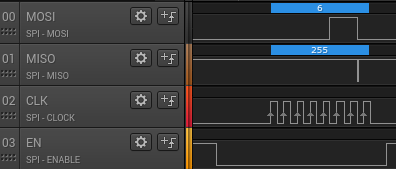
\includegraphics[scale=0.6]{coms_25lc640_start.png}
		\subcaption[first caption.]{Start of serial communication between the STM and the eeprom after when writing to the eeprom.}
		\label{fig:coms_25lc640_start}
	\end{minipage}
	\begin{minipage}[b]{\textwidth}
		\centering
		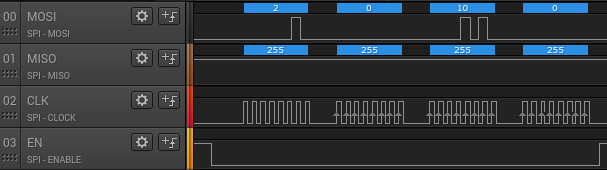
\includegraphics[scale=0.6]{coms_25lc640_data.png}
		\subcaption[second caption.]{End of serial communication between the STM and the EEPROM after when writing to the EEPROM.}
		\label{fig:coms_25lc640_data}
	\end{minipage}    
	\caption{Serial communication between the STM and the EEPROM after when writing to the EEPROM.}
	\label{fig:coms_25lc640}
\end{figure}
\subsubsection{Discussion}
Each group of instructions is sent when the enable (EN) line is pulled low and end when it is pulled high. The communication starts with a reset of the 25LC640 write enable latch as shown in  \cref{fig:coms_25lc640_start}. This operation consists of writing the \textit{WRDI (6)} instruction to the EEPROM. Following this is the write instruction and the data to be written sent on the MOSI line (\cref{fig:coms_25lc640_data}). Note that when data is being written to the device, only the MOSI line is active and the MISO line is in an impedance state observed as a logic 1 by the serial analyser. 

\subsection{HC-06}
The Bluetooth (HC-06) was tested by sending the string "abcdefg" to the Bluetooth device. The serial information generated by the STM Tx and Rx pins are displayed in \cref{fig:coms_hc-06}. As the Bluetooth device is receiving data, only the STM Tx line is displaying useful data. The analyser was set to interpret the UART protocol. The interpretation is display on the Tx line. 
\begin{figure}[h!]
	\centering
	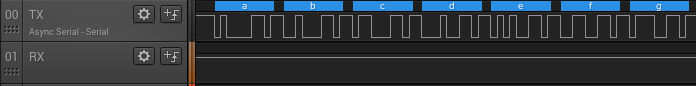
\includegraphics[scale=0.6]{coms_hc-06.png}
	\caption{Serial information received by the bluetooth device.}
	\label{fig:coms_hc-06}
\end{figure}
\subsubsection{Discussion}
The UART protocol is asynchronous and therefore does not use a clock; the data is sent continously as a stream of bits analysed in group of 8 to represent a character. The data sent matches what was expected. 

\subsection{NX4024T032\_001}
The nextion (NX4024T032\_001) was tested by sending the string "nextion" to the nextion device. The serial information generated by the STM Tx and Rx pins are displayed in \cref{fig:coms_nextion}. As the Bluetooth device is receiving data, only the STM Tx line is displaying useful data. The analyser was set to interpret the UART protocol. The interpretation is display on the Tx line. 
\begin{figure}[h!]
	\centering
	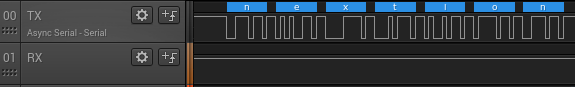
\includegraphics[scale=0.6]{coms_nextion.png}
	\caption{Serial information received by the nextion device.}
	\label{fig:coms_nextion}
\end{figure}
\subsubsection{Discussion}
The nextion touchscreen and the bluetooth device use the exact same protocol. The stream of data sent is correct. 

\subsection{WS2812}
The neopixels (WS2812) were tested by analysing the data sent by the STM. \Cref{fig:coms_ws2812_data} displays the encoded bit based on the Non-Return to Zero (NRZ) encoding used by the neopixels. \Cref{fig:coms_ws2812_low} displays 0 in NRZ while \cref{fig:coms_ws2812_high} displays 1 using the NRZ encoding. The timing information of the pulse generated by the STM are displayed on both figures.\\
To verify that the right information is sent to the neopixels, a stream of 24 PWM pulses, 8 per colour was sent to the neopixel in order to program the first pixel. The result of these tests are displayed in \ref{fig:coms_ws2812_colour}
\begin{figure}[h!]
	\centering
	\begin{minipage}[b]{\textwidth}
		\centering
		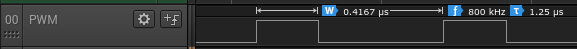
\includegraphics[scale=0.8]{coms_ws2812_low.png}
		\subcaption[first caption.]{Representation of 0 using the neopixel NRZ encoding.}
		\label{fig:coms_ws2812_low}
	\end{minipage}
	\begin{minipage}[b]{\textwidth}
		\centering
		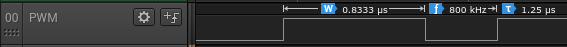
\includegraphics[scale=0.8]{coms_ws2812_high.png}
		\subcaption[second caption.]{Representation of 1 using the neopixel NRZ encoding.}
		\label{fig:coms_ws2812_high}
	\end{minipage}    
	\caption{Data sent to one neopixel to turn on specific colours.}
	\label{fig:coms_ws2812_data}
\end{figure}
\begin{figure}[h!]
	\centering
	\begin{minipage}[b]{\textwidth}
		\centering
		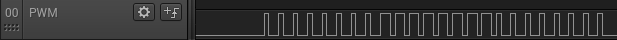
\includegraphics[scale=0.8]{coms_ws2812_red.png}
		\subcaption[first caption.]{Data sent to one pixel to turn on its red led.}
		\label{fig:coms_ws2812_red}
	\end{minipage}
	\begin{minipage}[b]{\textwidth}
		\centering
		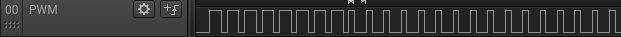
\includegraphics[scale=0.8]{coms_ws2812_green.png}
		\subcaption[second caption.]{Data sent to one pixel to turn on its green led.}
		\label{fig:coms_ws2812_green}
	\end{minipage}
	\begin{minipage}[b]{\textwidth}
		\centering
		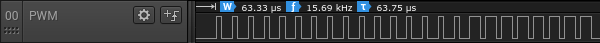
\includegraphics[scale=0.8]{coms_ws2812_blue.png}
		\subcaption[second caption.]{Data sent to one pixel to turn on its blue led.}
		\label{fig:coms_ws2812_blue}
	\end{minipage}    
	\caption{Data sent to one neopixel to turn on specific colours.}
	\label{fig:coms_ws2812_colour}
\end{figure}

\subsubsection{Discussion}
According to the WS2812 datasheet (see the documentation in \ref{npsc_harware}), the period of each code must be $ 1.25\mu s \pm 600ns$, looking at the codes in \ref{fig:coms_ws2812_data}, the STM achieves exactly a period of $1.25\mu s$. The datasheet specifies that the high time of code 1 should be $0.4\mu s \pm 0.15 \mu s$, the STM achieves a time of $0.42 \mu s$ which is in the range of the requirement. The high time of code 1 as per the datasheet should be $0.85 \mu s \pm 0.15 \mu s$, the time achieved is $0.833 \mu s$ which is also in the range of the required time. The codes generated by the STM to control the neopixels are in the right format.\\
Each neopixel requires a stream of 24 codes to be programmed. The first, second and third group of 8 codes represent respectively the 8bit value of the neopixel's green, red, and blue led. \Cref{fig:coms_ws2812_red}, \cref{fig:coms_ws2812_green}, and \cref{fig:coms_ws2812_blue} display the stream of 24 code setting the neopixel to red, green, and blue respectively. In \cref{fig:coms_ws2812_red}, it is expected to have code 0 for the first and last 8 pulses (green and blue) and code 1 for the second 8 pulses (red). The STM can send the correct stream to program the neopixels.

\subsection{Final comments on the hardware tests}
All tests performed on the hardware were successful, this is an indication that all modules work perfectly independently of any other modules. This is the basis for the test to be performed at a higher level of the hierarchy. However, some of the tests performed on the hardware are only focused on the STM sending the correct information to the device. Although this is a requirement for the communication to be established, the information received by the STM from the device should also be tested thoroughly. Moreover, these tests do not take into account other modules such as the sensors which use the STM analogue to digital converter.

%%%%%%%%%%%%%%%%%%%%%%%%%%%%%%%%%%%%%%%%%%%%%%%%%%%%%%%%%%%%%%%%%%%%%%%%%%%%%%%%%%%%
% SECTION: Software tests
%%%%%%%%%%%%%%%%%%%%%%%%%%%%%%%%%%%%%%%%%%%%%%%%%%%%%%%%%%%%%%%%%%%%%%%%%%%%%%%%%%%%
\section{Software Tests}
The results of all software tests performed on the NPSC are given in this section. It starts with the analysis of the unit tests followed by the result and analysis of the integration test. The last section is dedicated to the results and analysis of further tests and experiments performed in order to find the point of failure of some tests.

\subsection{Unit tests outcome}
The unit tests are sets of logical functions performed on specific hardware modules. After ensuring that the basic hardware tests have been passed, the following tests were run on the hardware framework. The outcome of the units tests run on the hardware and the coverage of the tests are given in \cref{table:software_unit_test}.
\begin{table}[h!]
	\centering
	\caption{Unit test outcome.}
	\label{table:software_unit_test}
	\begin{tabular}{cccc}
		\hline
		\hline
		\toprule
		\textbf{Hardware} & \textbf{Unit test} & \textbf{Outcome} & \textbf{Coverage}\\
		\bottomrule
		\toprule
		\multirow{3}{*}{internal RTC} & test\_clock\_date & Pass & \multirow{3}{*}{33.33\%}\\
		& test\_clock\_time & Pass &\\
		& test\_clock\_alarm & Pass &\\
		\midrule
		external RTC & test\_rtc\_clock & Pass & 47.1\%\\
		\midrule
		\multirow{3}{*}{queue} & test\_queue\_create & Pass & \multirow{3}{*}{44.44\%}\\
		& test\_queue\_enqueue & Pass &\\
		& test\_queue\_dequeue & Pass &\\
		\midrule
		\multirow{3}{*}{eeprom} & test\_eeprom\_write\_read & Pass & \multirow{3}{*}{66.67\%}\\
		& test\_eeprom\_write4B\_read4B & Pass &\\
		& test\_eeprom\_writeNB\_readNB & Pass &\\
		\bottomrule
		\hline
		\hline
	\end{tabular}
\end{table}
\subsubsection{Discussion}
\textbf{All unit tests designed for the hardware have passed.} This is an indication of the functioning of these hardware module at a logic level. This level is above the simple communication protocol verification between hardware. At this level, the logical operations performed on the hardware are perfomed. Note that the logic level hardware test require a positive outcome of the hardware communication tests.The coverage of the test is neither a line or statement coverage but a function coverage. For each test, the coverage is the ratio of the number of functions called by the module over the number of functions in the module as a percentage. A 33.33\% coverage indicates that only a third of the function in the module have been called. Therefore a low coverage is not an indication that the test did not cover all used functions of the module in the system.   

\subsection{Integration tests outcome}
The integration tests are designed to verify the functionalities of the applications. Unlike the unit tests, they are not specific to one framework but to one application. Each test is designed to suit the application are the logic of each application is different and complexed. The outcome and the coverage of the application test are given in \cref{table:software_integration_test}.
\begin{table}[h!]
	\centering
	\caption{Integration test outcome.}
	\label{table:software_integration_test}
	\begin{tabular}{cp{20em}cc}
		\hline
		\hline
		\toprule
		\textbf{Application} & \textbf{Test} & \textbf{Outcome} & \textbf{Coverage}\\
		\bottomrule
		\toprule
		\multirow{6}{*}{alarm} & test\_alarm\_address & Pass & \multirow{2}{*}{66.67\%}\\
		& test\_alarm\_save\_load & Pass &\\ 
		& Alarm to be triggered at a desired time and date & \multirow{2}{*}{Pass} & \multirow{2}{*}{N/A}\\ 
		& Alarm is loaded from EEPROM to either alarm A or B & \multirow{2}{*}{Pass} & \multirow{2}{*}{N/A}\\ 
		\midrule
		instruction & instruction\_execute & Pass & 100\%\\
		\midrule
		\multirow{3}{*}{visual} & Analyse neopixels data when all module are connected and compared to it to the expected data & \multirow{3}{*}{Fail} & \multirow{3}{*}{N/A}\\
		\bottomrule
		\hline
		\hline
	\end{tabular}
\end{table}
\subsubsection{Alarm}
The first test verifies that the address of each datatype of the AlarmTypeDef \footnote{Type definition of an alarm containing a label, a ringtone, a pattern, a time, a date, \ldots} used to store the alarm is correct. The second test verify that an alarm has been successfully saved in the EEPROM. Those two tests which covers 66.67\% of the code indicate that the interaction between the alarm application and the EEPROM is correct. Two other tests were performed on the application to ensure that the alarm type definition are actually set as alarm in either alarm A or B and are triggered accordingly. These two test are not automatic and therefore a their coverage cannot be given. \textbf{These test have shown that the alarm application works perfectly.}

\subsubsection{Instruction}
The instruction application test is similar to the hardware communication test. All functions in this application were tested under the \textit{instrcution\_execute} fucntions as it calls all other functions. The first set of instructions sent to the nextion screen after a clock request are displayed in \cref{fig:coms_instruction_nextion}.
\begin{figure}[ht]
	\centering
	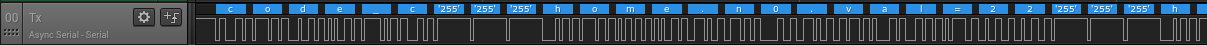
\includegraphics[scale=0.5]{coms_instruction_nextion.png}
	\caption{instruction sent to the nextion touchscreen to update the clock displayed on the screen.}
	\label{fig:coms_instruction_nextion}
\end{figure}
As explained in \ref{IFDE}, the STM communicate with the nextion touchscreen using a process consisting of three phases. The first phase (instruction\_nextionStart) consists of sending \textit{code\_c\"{y}\"{y}\"{y}} as seen in \cref{fig:coms_instruction_nextion}. The following information sent are instructions from the second phase of communication. \textbf{The instruction application is working according to its design.}

\subsubsection{Visual}
The visual application which relies mainly on the neopixels hardware failed. After performing some tests explained in \ref{visual_fail}, it was found that when all modules are activated, their interrupt service routines (ISR) pause the stream of data sent to the neopixels. The stream cannot be paused as it will be interpreted by the neopixels as two different streams. 

\subsection{Insight on Visual module integration failure}\label{visual_fail}
In order to understand the reason for the failure of the visual application, data was written to the neopixel every second. It takes $5.4ms$ to send information to 180 neopixels. Therefore sending the data every minute is largely sufficient to prevent the data from being overwritten. The data sent to the neopixels is shown in \cref{fig:test_neopixels}.
\begin{figure}[ht]
	\centering
	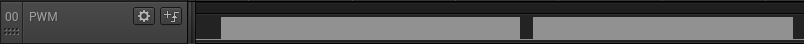
\includegraphics[scale=0.5]{test_neopixels.png}
	\caption{Corrupt data received by the Ring.}
	\label{fig:test_neopixels}
\end{figure}
As seen in \cref{fig:test_neopixels}, the data sent is being split in two. This means that a set of the 180 neopixels will receive data while the other will never receive data. This is the case because of the neopixels a daisy chain connection, as mentioned in the literature review, a delay of $5.53 ms$ (reset sequence) indicates the end of the transmission. Any data coming after a reset sequence will be interpreted as new data.\\
\textbf{What causes this?}\\
It is extremely hard to debug the system at this point as it is an ISR error. The tools provided by the free version of Atolic TrueSTUDIO are not sufficient to perform analytical tests on the ISR. However, the DMA was not used to send the information to the timer setting the PWM data. As a result, the CPU is responsible for fetching all the information from memory, which is a heavy workload. Moreover, it was realised that stream is stoped randomly but for a constant period of $127.1\mu s$. This is certainly due to another process having a higher priority than the neopixels timer. A fix to this problem might be to establish an ISR table an allocate priority according to the importance of each process.    

%%%%%%%%%%%%%%%%%%%%%%%%%%%%%%%%%%%%%%%%%%%%%%%%%%%%%%%%%%%%%%%%%%%%%%%%%%%%%%%%%%%%
% SECTION: Ring 
%%%%%%%%%%%%%%%%%%%%%%%%%%%%%%%%%%%%%%%%%%%%%%%%%%%%%%%%%%%%%%%%%%%%%%%%%%%%%%%%%%%%
\section{Ring experiments}
The Ring, being made out of many neopixels,  is considered as a huge neopixel referred to the NeoPixel in this section. The experiments performed on the Ring are therefore to quantify the characteristics of this neopixel. This section aims to provides mathematical expressions of the NeoPixel's temperature rise, current drawn, and illuminance.

\subsection{Current drawn by the Ring}
\textbf{Requirement:}  \textit{The NeoPixel must be able to withstand a current of $10.8A$.}\\
In order to evaluate the performance of the NeoPixel, three sub-experiments were performed on it. The first experiment quantifies the current drawn by a single neopixel in the Ring per brightness and colour. The second experiment provides an approximation of the NeoPixel idle current. As for the third experiment provides an estimation of the NeoPixel's current per brightness level.

\subsubsection{Current drawn by one neopixel} \label{current_one}
The current drawn by a single neopixel per colour and brightness level is graphically represented by \cref{fig:current_one_pixel}. The current drawn per red, green and blue led is represented respectively by the plot of the colour red, green, and blue. The current drawn by a single neopixel with all its colours set at the same brightness is represented by the black plot (RBG). The figure also provides the best fit line equation as well as the correlation between the best fit line and the plot.  
\begin{figure}[ht]
	\centering
	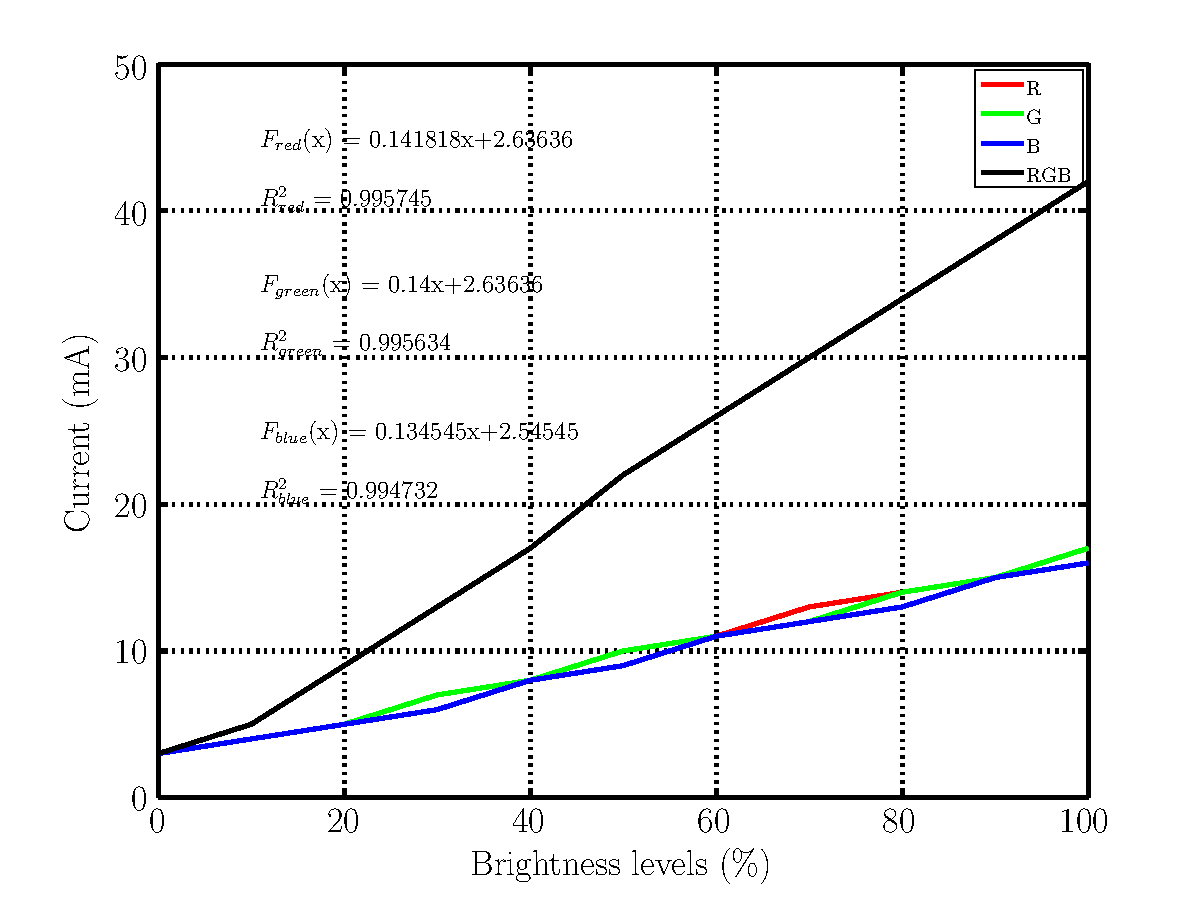
\includegraphics[scale=0.6]{current_one_pixel.pdf}
	\caption{Current drawn by a one neopixel per colour at different brightness levels.}
	\label{fig:current_one_pixel}
\end{figure}
The currents drawn by each led in the neopixel differ by at most $1mA$. They follow the same trend which is expected although the neopixel datasheet does not provide the current consumption of each led. The mathematical relationship between the current drawn by each led colour and its brightness are given by :
\begin{equation}
\label{eq:f_red}
\begin{multlined}
f_{red}(x) = 0.141818x+2.63636 \\
r^2_{red} = 0.995745
\end{multlined}
\end{equation} 
\begin{equation}
\label{eq:f_green}
\begin{multlined}
f_{green}(x) = 0.14x+2.63636 \\
r^2_{green} = 0.995634
\end{multlined}
\end{equation} 
\begin{equation}
\label{eq:f_blue}
\begin{multlined}
f_{blue}(x) = 0.134545x+2.54545 \\
r^2_{blue} = 0.994732
\end{multlined}
\end{equation} 
{
	\centering
	\textit{$x$ is the brightness in \%}\\
}

The correlations between the \cref{eq:f_red,eq:f_green,eq:f_blue} and the plots in \cref{fig:current_one_pixel} are very strong. Each led has a idle current of $2.6 \pm 0.052487 mA$ and consume up $16.485 \pm 0.42964 mA$. The maximum current drawn by each led is $3.515\pm0.430 mA$ less than the current provided by the datasheet. The new expected current drawn by the NeoPixel is:\\

{
	\centering
	Led current = $16.485 \pm 0.4296 mA$ \\
	Removing the microcontroller current from the result,\\ the actual led current = $16.485 \pm 0.4296 mA - 2.6 \pm 0.0525 mA = 13.885 \pm 0.3771$  \\
	Total leds current = $(13.885 \pm 0.377)*3 = 41.655 \pm 1.131 mA$  \\
	one neopixel current = $41.655 \pm 1.131 mA + 2.6 \pm 0.0525 mA  = 44.255 \pm 1.184 mA $\\
	\textbf{Estimated NeoPixel current} = $7.966 \pm 0.213 A$\\
}
This estimation is $2.834\pm0.213A$ less than the board current requirement.

\subsubsection{Idle current of the NeoPixel}\label{idle_current}
The idle current of the NeoPixel per neopixels receiving data is shown in \cref{fig:current_idle}. This result was obtained by taking eight sample listed in \cref{table:current_idle}. 
\begin{figure}[ht]
	\centering
	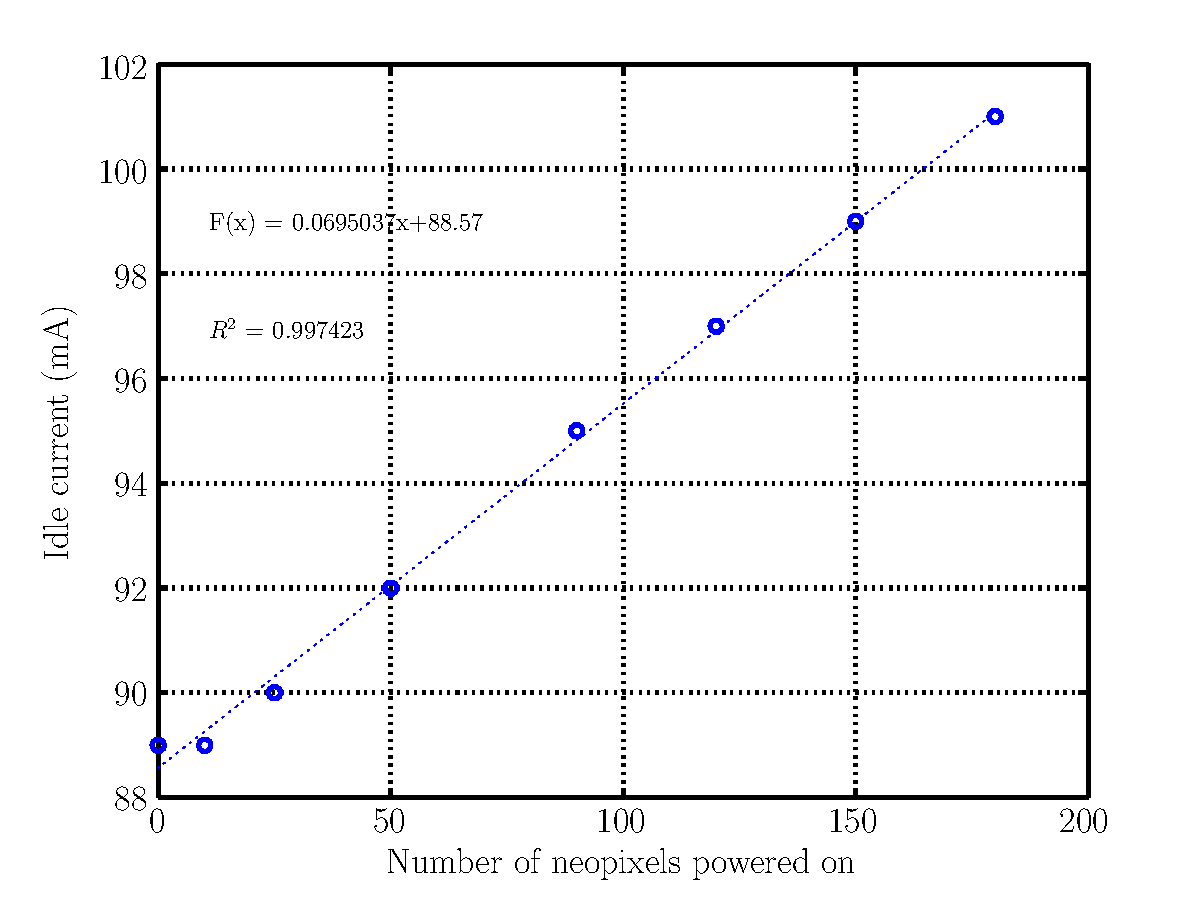
\includegraphics[scale=0.6]{current_idle.pdf}
	\caption{Idle current of the NeoPixel per neopixels receiving power off data.}
	\label{fig:current_idle}
\end{figure}
The idle current increases linearly as the number of neopixels receiving power off data \footnote{power off data is defined as the 24 code 0 indicating that all led should be turned off} increases. This relationship is given by 
\begin{equation}
\label{eq:f_idle}
\begin{multlined}
f(x) = 0.0695x+88.57 \\
r^2 = 0.9974\\
\textit{$x$: number of neopixels}
\end{multlined}
\end{equation} 
From \cref{eq:f_idle}, the NeoPixel is expected to have a idle current of $101.08mA$. The result shows that when no data is sent at all to the NeoPixel, it still draws a current of $88.57mA$. The neopixels each have a microcontroller, analysing the coming data and setting the brightness level of each led accordingly. When no data is sent to the neopixels, their microcontroller is still powered. Since no LEDs are turned on, the NeoPixel's minimum idle current of $88.57mA$ is the current drawn by each neopixel in the Ring. From \cref{eq:f_idle}, the idle current increases as the number of neopixel receiving power off data increases. This result is expected as each microcontroller has to do more processing as the number of neopixel increases. 

\subsubsection{Current drawn by the NeoPixel}\label{current_180}
The current drawn by the NeoPixel (ring of 180 neopixels) is graphically represented in \cref{fig:current_180_neopixels}. All red, green, and blue LEDs were set to the same brightness level to reduce the complexity of the experiment. The current values were obtained by averaging the results of three sample per brightness as shown in \cref{table:current_180_neopixels}. 
\begin{figure}[ht]
	\centering
	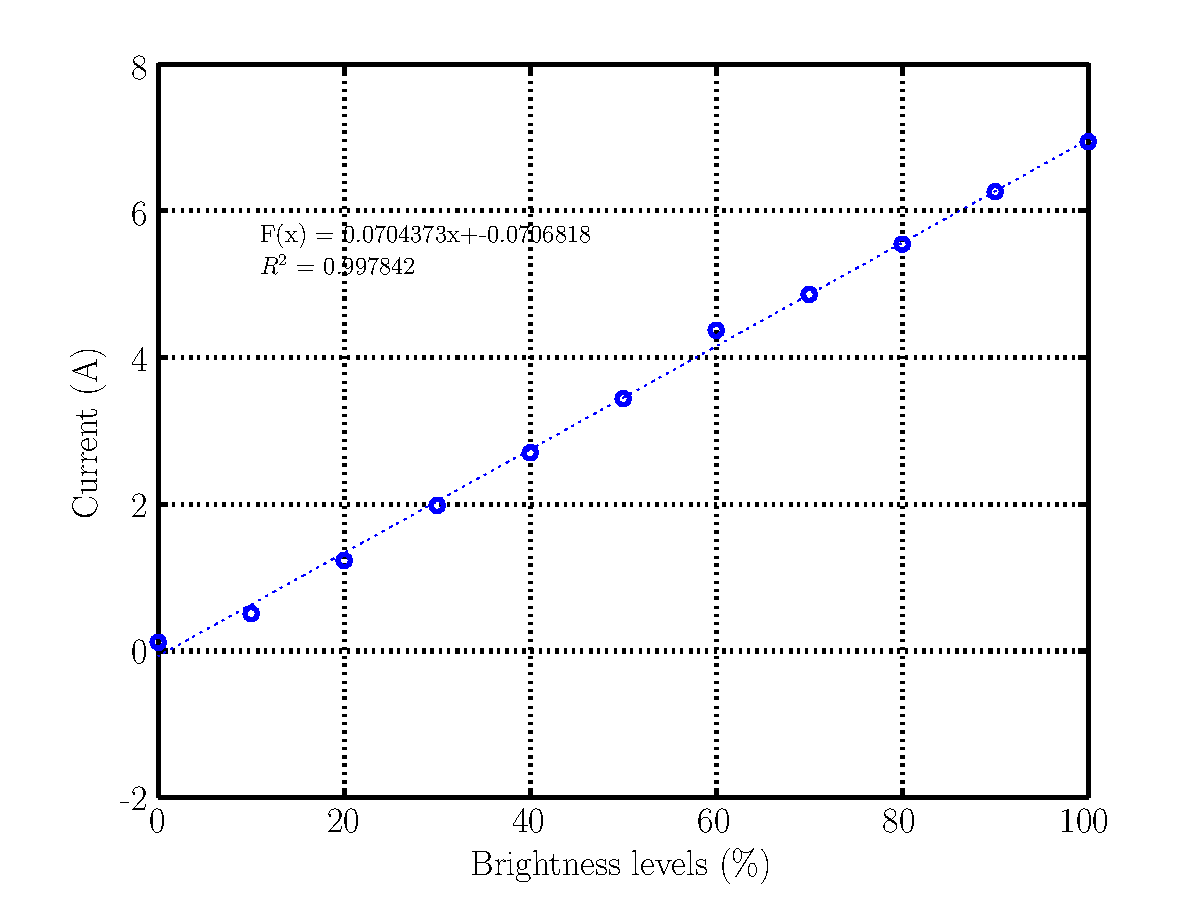
\includegraphics[scale=0.6]{current_180_neopixels.pdf}
	\caption{Current drawn by all 180 neopixels on the Ring at different brightness levels.}
	\label{fig:current_180_neopixels}
\end{figure}
The plot has a linear trend given by:
\begin{equation}
\label{eq:f_180}
\begin{multlined}
f(x) = 0.07043x-0.0707 \\
r^2 = 0.9978\\
\textit{$x$: brightness level}
\end{multlined}
\end{equation} 
The mathematical model provided by \cref{eq:f_180} is bounded by $0A$ and $6.9723A$. Using the table used to find this model, the NeoPixel has an idle current of $0.12A$ and a maximum current of $6.94A \pm 0.08 A$. The idle current is more than the one obtained in \cref{idle_current} by $0.031A$. The maximum current drawn by the NeoPixel at full brightness of all its leds is $7.020A$, this is $3.78A$ less than the expected current drawn. Obtaining a smaller current drawn by the NeoPixel compared to the one calculated from the datasheet  was expected after analysis of the results in \cref{current_one}. The experimental current drawn by the NeoPixel is less than the second theoretical estimation by $0.946A$.

\subsubsection{Overal discussion}
The experiments done to estimate the current drawn by the NeoPixel provided interesting results. Each led draws the same current per brightness level. The microcontroller of each neopixel draws a small amount of current defined as the neopixel's idle current. The NeoPixel itself draws $6.94A \pm 0.08 A$ which is $3.78A$ less than the theoretical current.\\
\textbf{The NeoPixel draws less than 10.8A}


\subsection{Ring temperature}
\textbf{Expectation:} \textit{The Ring should have a temperature rise of $15^oC$}.\\
The temperature rise of the Ring is graphically represented by \cref{fig:temperature_ring}. The temperature was taken per brightness level, however, it was judged more useful to have a relationship between the Ring's temperature and its current drawn. 
\begin{figure}[ht]
	\centering
	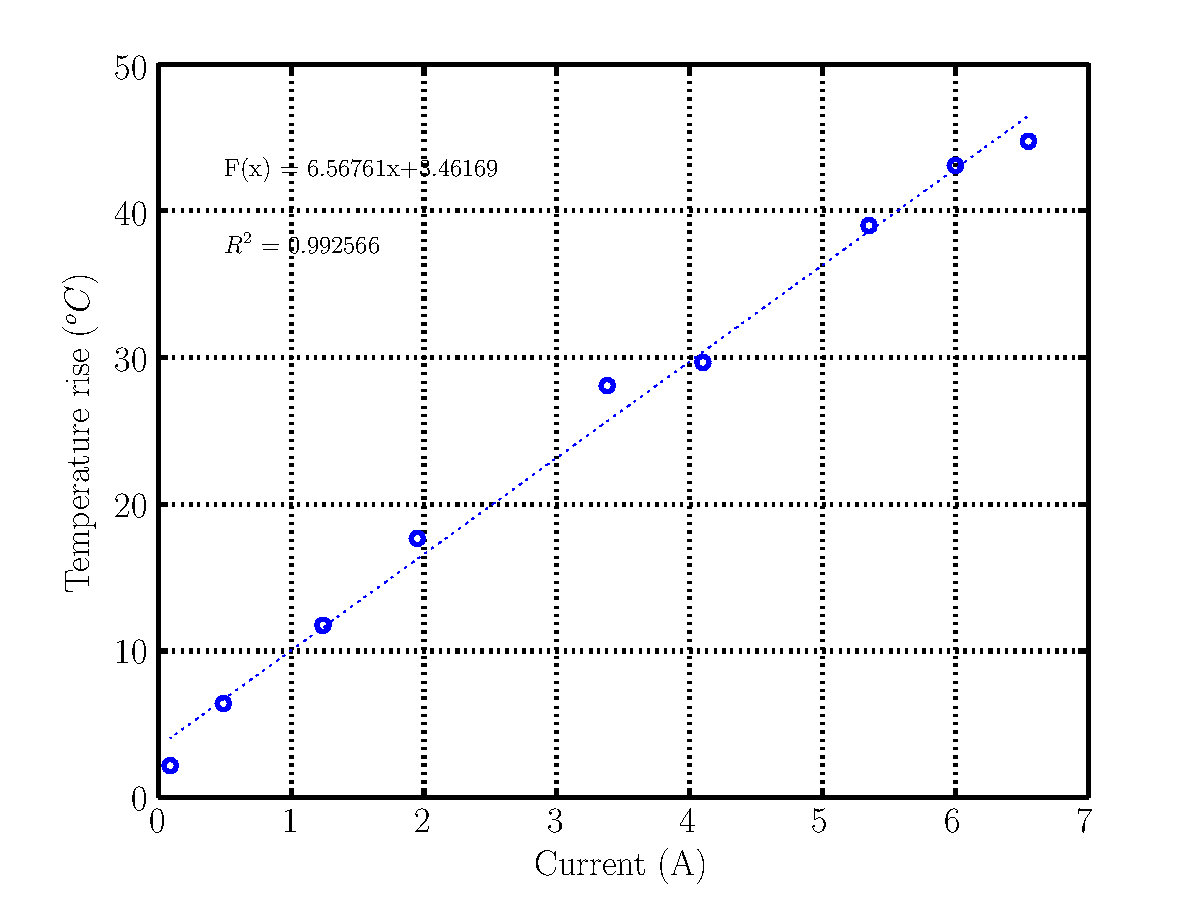
\includegraphics[scale=0.6]{temperature_ring.pdf}
	\caption{Ring's temperature rise.}
	\label{fig:temperature_ring}
\end{figure}

\subsubsection{Discussion}
The temperature rise varies from $2.176^oC$ to $44.75^oC$. The lowest temperature rise is the one value corresponding to the idle state of the NeoPixel. As for the highest temperature represent the temperature rise of the NeoPixel at full brightness of all its LEDs. The mathematical model of the temperature rise is given by the linear equation:
\begin{equation}
\label{eq:f_temp}
\begin{multlined}
f(x) = 6.568x+3.462 ^oC\\
r^2 = 0.9927\\
\textit{$x$: current (A)}
\end{multlined}
\end{equation}  
The temperature rise obtained is way above what the board was designed for. In \cref{ring_pcb}, it predicted that the board temperature will exceed what it was designed for due to the mechanical constraint of the Ring. \\
Another observation was made on the effect of the board temperature on the current drawn. The current listed in \cref{table:current_180_neopixels,table:temperature_ring} varies significantly. In the result obtained in \cref{current_180}, the temperature in \cref{table:current_180_neopixels} decreases as more sample are taken. It is known that the resistivity os a wire increases as the wire temperature increases. Moreover, the relation between current and voltage is given by $I=\frac{V}{R}$. Based on these relationships, an increase in the board temperature will result in an increase of the board resistivity resulting in an increase of the track resistivity. As the Ring is supplied with a constant voltage of $5V$, an increase in the track resistance results in a decrease of the board's current drawn, which is observed in these experiments.\\

\subsection{Illuminance produced by the Ring}
\textbf{Requirement:}  \textit{The NeoPixel must be able to emit light of $460\pm 10 nm$ wavelength with an illuminance of $30lx$.}\\
The results of the experiments are sectioned into two categories, the illuminance of the blue led, and the relationship between the NeoPixel illuminance and the distance and angle to the normal of the NeoPixel's surface. Because the NeoPixel uses a space of $21*21cm^2$, it was considered as a semisphere with a radius of $21cm$. For this reason, the results obtained at a distance of less than 20cm were discarded as not all neopixel's light would be received by an object inside the semi-sphere described.\\
All the results obtained for the experiment are shown in \cref{appendix_result}.

\subsubsection{Blue light illuminance}\label{illuminance_blue}
The blue led on the neopixel have a wavelength of $465-467nm$ and are the only led whose wavelength is in the range of $460\pm 10 nm$. The illuminance-distance relationship was observed at full blue light brightness at 0, 30, 60, and 90 degrees and is graphically represented in \cref{fig:illuminance_distance}. 
\begin{figure}[ht]
	\centering
	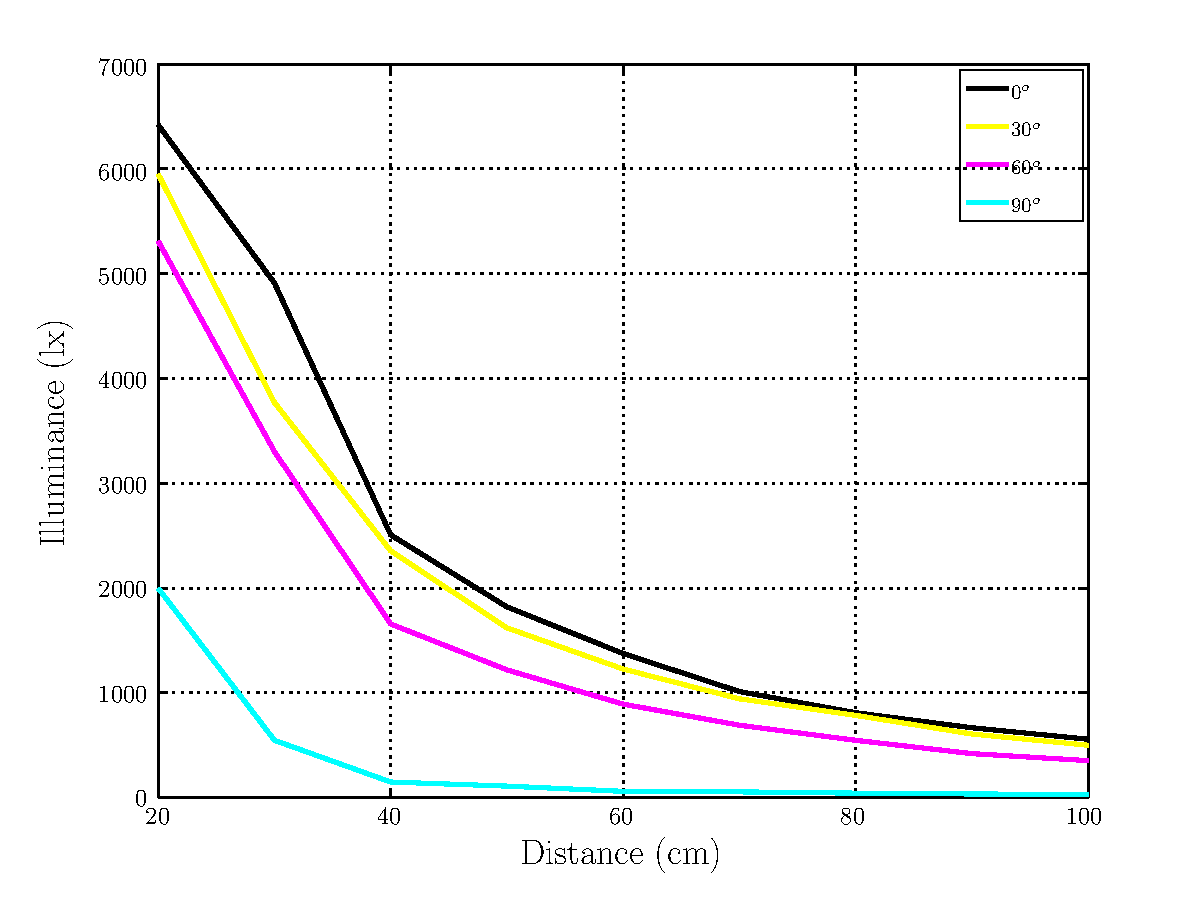
\includegraphics[scale=0.6]{illuminance_blue.pdf}
	\caption{Ring's blue LED illuminance at full brightness per distance and angular section to the Ring.}
	\label{fig:illuminance_blue}
\end{figure}
The illuminance decreases exponentially as the distance increases. The maximum illuminance of $6420lx$ is obtained at a distance of 20cm away from the normal to the NeoPixel's surface. The minimum illuminance $30lx$ is obtained at any object located 100cm away and at an angle of 90 degrees to the NeoPixel's surface. Any object located in the semi-circle of radius 100cm with the NeoPixel at the centre of the semi-circle and facing the described region will receive a minimum of $30lx$. \\
Based on \cref{eq:illuminance}, the NeoPixel blue light is supposed to have an illuminance of $32.4lx$ at a distance of 100cm. However, the NeoPixel's illuminance at 100cm in the experiment performed is $557lx$. Although the behaviour of the plots in \cref{fig:illuminance_blue} is expected, the illuminance of the NeoPixel is 17 time the expected illuminance. \\
To understand this difference, the lux meter used for the experiment was compared to other types of lux meter available on smartphones. The result obtained by these lux meters were similar. The room used for the experiment was completely dark and the lux meter's reading was $0lx$ before the NeoPixel was turned on. A possible reason is the reflection in the room. The NeoPixel was placed on white tables and the light was certainly reflected from the table to the lux meter increasing its reading.    

\subsubsection{Relationship between illuminance and distance to the board}
The result focuses on the relationship between the distance to the NeoPixel and the illuminance. To obtained the data of interest, the illuminance of the NeoPixel tabulated in \cref{table:illuminance_distance_value} at certain distances was converted into a ratio. This ratio is obtained by dividing the illuminance obtained at any distance by the illuminance at 20cm. The relationship between the illuminance and the distance to the board is graphically represented by \cref{fig:illuminance_distance}.
\begin{figure}[ht]
	\centering
	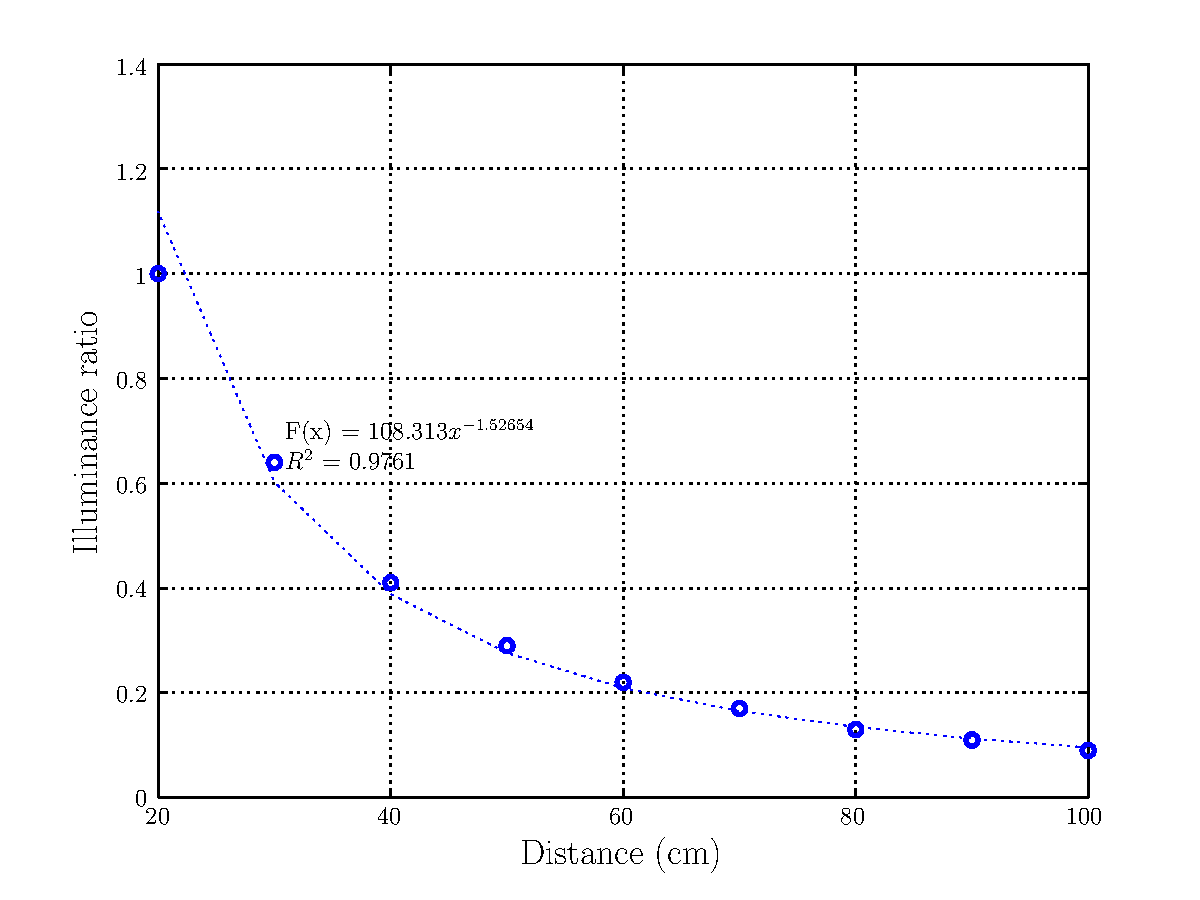
\includegraphics[scale=0.6]{illuminance_distance.pdf}
	\caption{Relationship between the coefficient of decadence of the Ring's illuminance and the distance to the Ring.}
	\label{fig:illuminance_distance}
\end{figure}
The plot obtained by \cref{fig:illuminance_distance} has a exponential trend given by:
\begin{equation}
\label{eq:f_distance}
\begin{multlined}
f(x) = 108.313x^{-1.52654} \\
r^2 = 0.9761\\
\textit{$x$: Distance (cm)}
\end{multlined}
\end{equation} 
According to \cref{eq:illuminance}, the illuminance is inversly proportional to the square of the distance in meter. It is relatedd to the NeoPixel in the following way (see \cref{appendix_equation}):\\
{
	\centering    
	\[g(x) = 400x^{-2}\]\\
	\textit{x: Distance (cm)}\\
}
The difference between this theoretical equation and the experimental mathematical model is illustrated in \cref{fig:illuminance_corr}. The two graphs have a correlation of 99.62\% indicating that the experimental model is accurate. The difference the plot's illuminance ratio is due to the errors in the experimental model as mentioned in \cref{illuminance_blue}. 
\begin{figure}[ht]
	\centering
	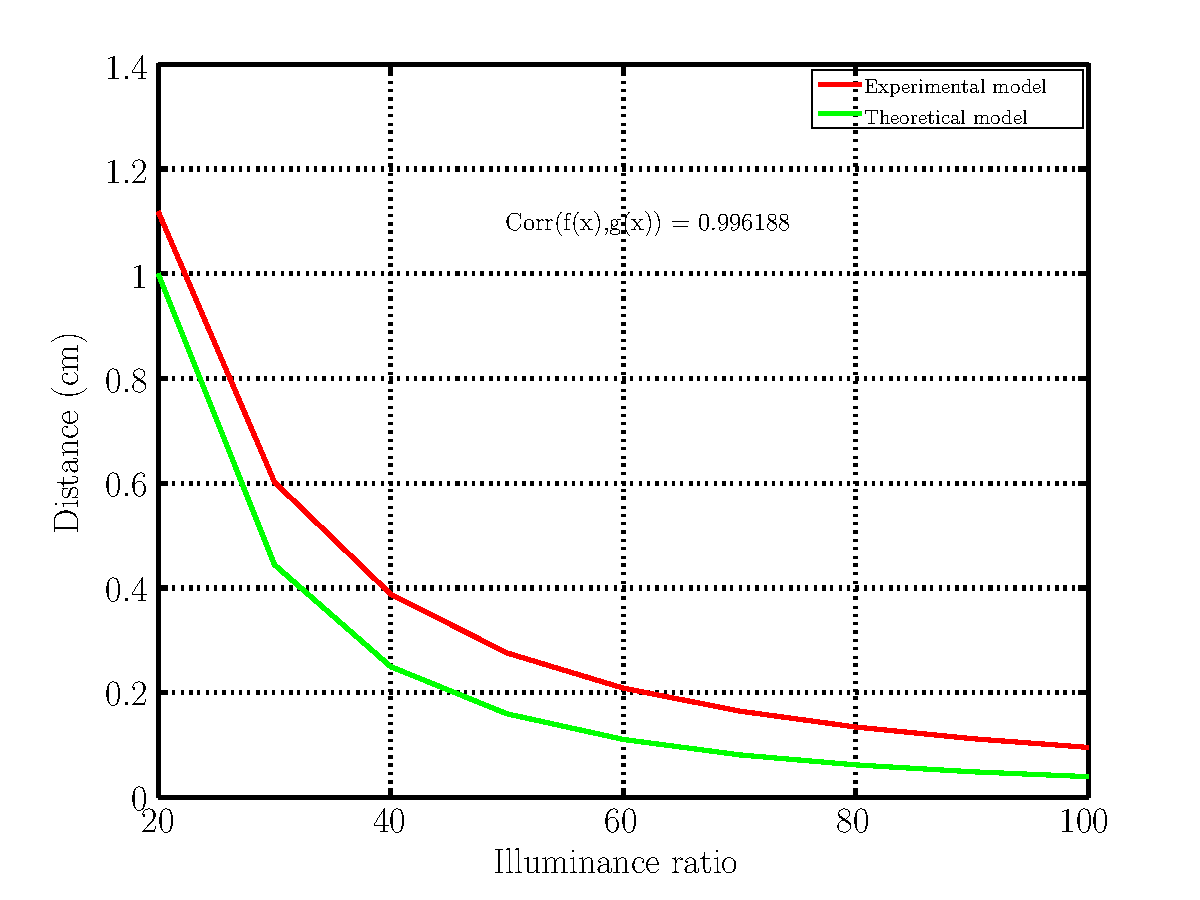
\includegraphics[scale=0.6]{illuminance_corr.pdf}
	\caption{Experimental vs theoretical relationship between illuminance and distance.}
	\label{fig:illuminance_corr}
\end{figure}

\subsubsection{Relationship between illuminance and angle of positionement}
The result focuses on the relationship between the angle to the NeoPixel and the illuminance. To obtained the data of interest, the illuminance of the NeoPixel at certain angle was converted into a ratio. This ratio is obtained by dividing the illuminance obtained at any angle by the illuminance at an angle of 0 degrees. The relationship between the illuminance and the angle to the normal of the NeoPixel surface is graphically represented by \cref{fig:illuminance_angle}.
\begin{figure}[ht]
	\centering
	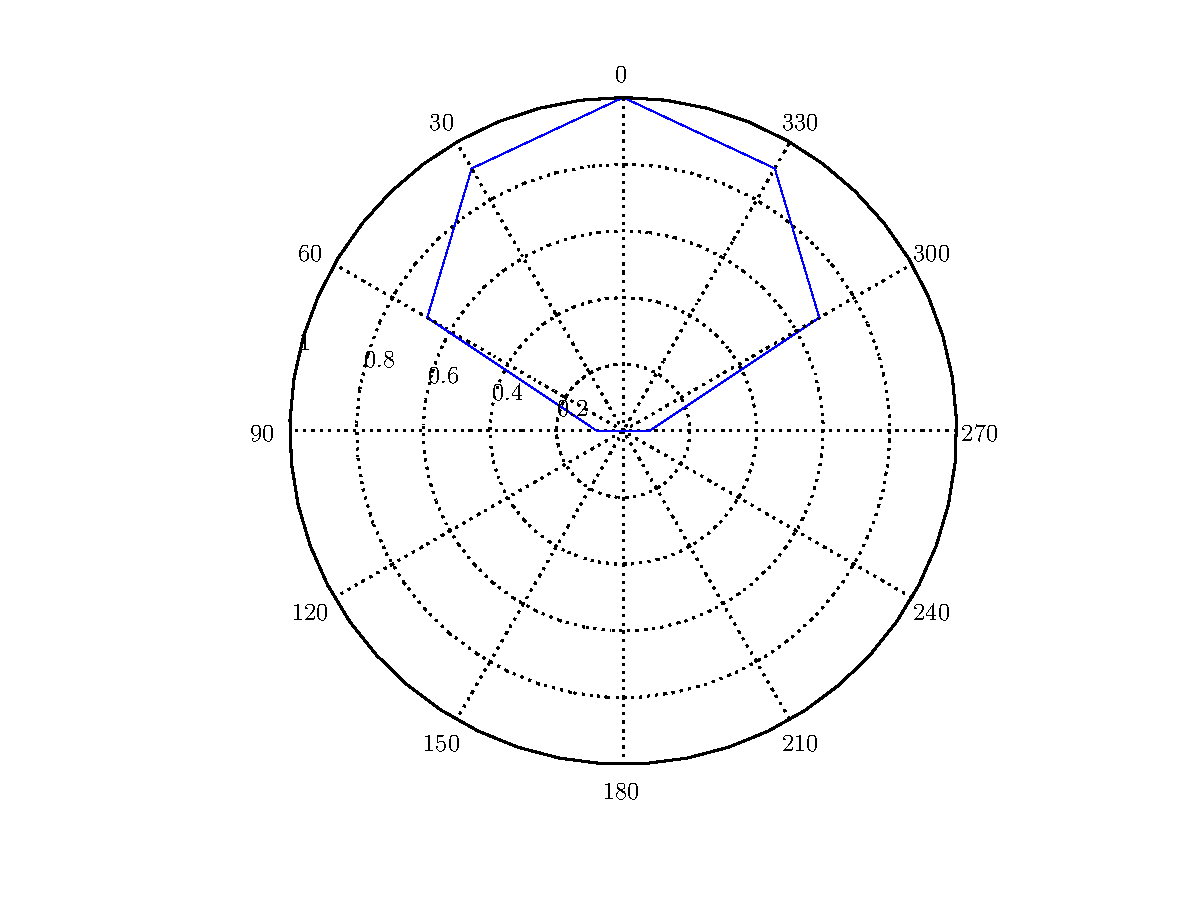
\includegraphics[scale=0.6]{illuminance_angle.pdf}
	\caption{Relationship between the Ring illuminance and the angle to the normal of the Ring surface.}
	\label{fig:illuminance_angle}
\end{figure}
The illuminance decreases as the angle to the normal of the NeoPixel surface increases. Any objects in front of the NeoPixel will receive an illuminance. However, any object behind the NeoPixel will not. This model follows Lambert's Cosine law given by \cref{eq:lambert}. To maximise the illuminance, the object must be on the normal to the surface of the NeoPixel.

\subsubsection{Conclusion of these experiment}
The NeoPixel has the following characteristics:
\begin{itemize}
	\item The illuminance received by an object decreases as the is moved further away from the NeoPixel.
	\item The illuminance received by an object decreases as the is moved at an angle further away from the normal of the NeoPixel.
	\item \textbf{The NeoPixel produces at least 30lx on any object placed in front of the neopixel at a maximum distance of 1m.}
\end{itemize}